\documentclass[12pt]{beamer}
\usepackage[utf8]{inputenc}
\usepackage{listings}
\usepackage{tabu}
\beamertemplatenavigationsymbolsempty
\AtBeginSection[]
{
    \begin{frame}
    \frametitle{Table of Contents}
    \tableofcontents[currentsection]
    \end{frame}
}
\lstset{language=C++, basicstyle=\footnotesize, frame=single}

\title{Number theory}
\subtitle{Prime factors, sieve, GCD, extended Euclid}
\author{beCP Training}
\institute{
\includegraphics[height=12em]{../share/beoi-logo}}

\begin{document}

\frame{\titlepage}

\section{Prime check}

\begin{frame}
\frametitle{Prime numbers}
\[2,\ 3,\ 5,\ 7,\ 11,\ 13,\ 17,\ 19,\ 23,\ldots\]
\begin{itemize}
\item Prime numbers have exactly two divisors: 1 and themselves
\item Numbers with three or more are called \emph{composite}
\item We can decompose any number into a product of primes
\item This decomposition is \emph{unique}
\end{itemize}

~

Examples:
\[ 6 = 2 \cdot 3 \qquad 8 = 2^3 \qquad 45 = 3^2 \cdot 5 \qquad 13 = 13 \]
\end{frame}

\begin{frame}[fragile]
\frametitle{Prime check: linear}
\begin{itemize}
\item How to check if $n$ is prime?
\item By checking that only 1 and $n$ divide $n$.
\end{itemize}

~

\textbf{Solution 1:} $O(n)$
\begin{lstlisting}
bool isPrime(int n)
{
    for (int i = 2; i < n; i++)
        if (n % i == 0)
            return false;
    return true;
}
\end{lstlisting}
Note: we will ignore 0 and 1 here.
\end{frame}

\begin{frame}[fragile]
\frametitle{Prime check: stop at square root}
\begin{itemize}
\item Actually, if $d$ divides $n$, then $n/d$ too
\item Since $d \times n/d = n$, at least one of them is $\leq \sqrt{n}$
\item So we only need to check up to $\sqrt{n}$
\end{itemize}
~

\textbf{Solution 2:} $O\left(\sqrt{n}\right)$
\begin{lstlisting}
bool isPrime(int n)
{
    for (int i = 2; i*i <= n; i++) // changed
        if (n % i == 0)
            return false;
    return true;
}
\end{lstlisting}
\end{frame}

\begin{frame}[fragile]
\frametitle{Factorization}
\begin{itemize}
\item We can also factor a number with this trick
\item If there are factors missing when reaching the square root, the remainder is prime
\end{itemize}

\begin{lstlisting}
vector<int> factors(int n)
{
    vector<int> f;
    for (int i = 2; i*i <= n; i++) {
        while (n % i == 0) {
            f.push_back(i);
            n /= i;
        }
    }
    if (n != 1) f.push_back(n); // n is prime now
    return f;
}
\end{lstlisting}
\end{frame}

\section{Sieve of Eratosthenes}

\begin{frame}
\frametitle{Sieve idea}
\begin{itemize}
\item What if we want to factorize many numbers?
\item Going up to $\sqrt{n}$ for all is slow
\end{itemize}

~

Idea: go through the numbers one by one
\begin{itemize}
\item If not prime, skip it
\item If prime, mark its multiples as not prime
\end{itemize}
\end{frame}

\newcommand{\g}[1]{\only<#1->{\color{gray}}\only<#1>{\color{red}}}
\begin{frame}
\frametitle{Sieve example}
{\tabulinesep=7pt
\begin{tabu}{cccccccccccc}
\g{1}1&\only<2>{\bf}{2}&\only<3>{\bf}3&\g{2}4&\only<4>{\bf}5&\g{2}6&\only<5>{\bf}7&\g{2}8&\g{3}9&\g{2}10&11&\g{2}12\\
13&\g{2}14&\g{3}15&\g{2}16&17&\g{2}18&19&\g{2}20&\g{3}21&\g{2}22&23&\g{2}24\\
\g{4}25&\g{2}26&\g{3}27&\g{2}28&29&\g{2}30&31&\g{2}32&\g{3}33&\g{2}34&\g{4}35&\g{2}36\\
37&\g{2}38&\g{3}39&\g{2}40&41&\g{2}42&43&\g{2}44&\g{3}45&\g{2}46&47&\g{2}48\\
\g{5}49&\g{2}50&\g{3}51&\g{2}52&53&\g{2}54&\g{4}55&\g{2}56&\g{3}57&\g{2}58&59&\g{2}60\\
61&\g{2}62&\g{3}63&\g{2}64&\g{4}65&\g{2}66&67&\g{2}68&\g{3}69&\g{2}70&71&\g{2}72\\
73&\g{2}74&\g{3}75&\g{2}76&\g{5}77&\g{2}78&79&\g{2}80&\g{3}81&\g{2}82&83&\g{2}84\\
\g{4}85&\g{2}86&\g{3}87&\g{2}88&89&\g{2}90&\g{5}91&\g{2}92&\g{3}93&\g{2}94&\g{4}95&\g{2}96\\
\end{tabu}}
\end{frame}

\begin{frame}[fragile]
\frametitle{Sieve implementation}
\begin{lstlisting}
typedef long long ll; // to avoid overflow on i*i
bitset<MAXN> bs; bs.set(); // set to true
vector<int> primes;

for (ll i = 2; i < MAXN; i++) {
    if (bs[i]) {
        // We can start it i*i
        for (ll j = i*i; j < MAXN; j += i)
            bs[j] = false;
        primes.push_back((int) i);
    }
}
\end{lstlisting}
\begin{itemize}
\item Complexity: $O(n \log \log n)$ (because math)
\item Practical limit: 1M $\sim$ 10M
\end{itemize}
\end{frame}

\begin{frame}[fragile]
\frametitle{Prime check with sieve}
\begin{itemize}
\item If $n < \mathsf{MAXN}$, use the table, $O(1)$
\item If $n < \mathsf{MAXN}^2$, use the prime list
\item Complexity is $O(\sqrt{n}\,/\log n)$ because the density of primes is proportional to $1\,/ \log n$
\end{itemize}
\begin{lstlisting}
// Only called for n < (last prime)^2
bool isPrime(int n)
{
    if (n < MAXN)
        return bs[n];
    for (int i=0; primes[i]*primes[i] <= n; i++)
        if (n % primes[i] == 0)
            return false;
    return true;
}
\end{lstlisting}
\end{frame}

\begin{frame}[fragile]
\frametitle{Sieve variants}
We can get additional information from the sieve:
\begin{itemize}
\item A way to get the factorization very quickly, $O(\log n)$
\item The number distinct prime factors
\end{itemize}
\begin{lstlisting}
int numDiffPF[MAXN], largestPF[MAXN]; // init to 0

for (ll i = 2; i < MAXN; i++) {
    if (numDiffPF[i]) {
        // This time we must start at i
        for (ll j = i; j < MAXN; j += i) {
            numDiffPF[j]++;
            largestPF[j] = i;
        }
    }
}
\end{lstlisting}
Divide by largestPF recursively to find factorization.
\end{frame}

\section{Greatest Common Divisor}

\begin{frame}
\frametitle{GCD definition}
The \emph{greatest common divisor} of $a$ and $b$ is the largest number that divides $a$ and $b$.

~

Examples:
\[\gcd(4,6) = 2 \quad \gcd(7,5) = 1 \quad \gcd(24,12)=12\]
\[\gcd(n,n) = n \quad \gcd(n,0) = n \quad \gcd(n,1) = 1\]

~

When using the factorization, just take the minimum of the exponents ($p^0$ is implied):
\[\gcd(2^5\cdot3^2,\ 2^4\cdot3^7) = 2^4\cdot3^2 \qquad \gcd(5^2, 3^5) = 1\]
\end{frame}

\begin{frame}
\frametitle{Euclid for GCD}
\begin{itemize}
\item Interesting property: $\gcd(a,b) = \gcd(a+bn,b)$
\item In particular: $\gcd(a, b) = \gcd(a\,\%\,b, b)$
\item So we can always reduce the problem to a smaller pair!
\end{itemize}

~

\begin{itemize}
\item Example:
\begin{center}$21 \quad 15 \quad 21\,\%\,15=\fbox{6} \quad 15\,\%\,6=\fbox{3} \quad 6\,\%\,3=\fbox{0} $\end{center}
\item The pairs are $(21,15)$, $(15,6)$, $(6,3)$, $(3,0)$.
\item We know that $\gcd(3,0) = 3$, so $\gcd(21,15) = 3$.
\end{itemize}
\end{frame}

\begin{frame}[fragile]
\frametitle{GCD implementation}
\textbf{Solution:} Euclid's algorithm
\begin{lstlisting}
int gcd(int a, int b)
{
    if (b == 0) return a;
    return gcd(b, a%b);
}
\end{lstlisting}
\begin{itemize}
\item Extremely simple
\item Exercise: prove that after two iterations $b$ is divided by at least 2 (hint: separate $a\,\%\,b \leq b/2$ and $a\,\%\,b > b/2$)
\item Complexity: $O(\log b)$
\end{itemize}
\end{frame}

\newcommand{\lcm}{\mathsf{lcm}}

\begin{frame}
\frametitle{Least Common Multiple}
The \emph{least common multiple} of $a$ and $b$ is the smallest number divisible by $a$ and $b$.

It is the ``opposite'' of the GCD.

~

Examples:
\[\lcm(4,6) = 12 \quad \lcm(7,5) = 35 \quad \lcm(24,12)=24\]
\[\lcm(n,n) = n \quad \lcm(n,0) = n \quad \lcm(n,1) = n\]

~

When using the factorization, just take the \emph{maximum} of the exponents:
\[\lcm(2^5\cdot3^2,\ 2^4\cdot3^7) = 2^5\cdot3^7 \qquad \lcm(5^2, 3^5) = 3^5\cdot5^2\]
\end{frame}

\begin{frame}[fragile]
\frametitle{Getting LCM from GCD}
\begin{itemize}
\item The GCD takes the minimum of the exponents and the LCM takes the maximum
\item So they take both exponents!
\item As a consequence, $\gcd(a,b) \times \lcm(a,b) = a \times b$
\end{itemize}

Example:
\[\gcd(2^5\cdot3^2,\ 2^4\cdot3^7) = 2^4\cdot3^2 \quad\ \lcm(2^5\cdot3^2,\ 2^4\cdot3^7) = 2^5\cdot3^7\]
\[\gcd\times\,\lcm = 2^{4+5}\cdot3^{2+7} = (2^5\cdot3^2) \times (2^4\cdot3^7)\]

~

\textbf{Solution:} Just be careful with overflows!
\begin{lstlisting}
int lcm(int a, int b) { return a * (b / gcd(a,b); }
\end{lstlisting}
\end{frame}

\section{Extended Euclid}

\newcommand{\di}{\,|\,}

\begin{frame}
\frametitle{Linear diophantine equation}
\begin{itemize}
\item A diophantine equation is an equation where the solutions must be integers
\item We will consider the equation $ax+by=c$ ($x,y$ unknown)
\item Note: if we had $x,y \in \mathbb{R}$ the solution would be a line
\item Let $d = \gcd(a,b)$. Since $d$ divides $ax+by$, it must also divide $c$.
\end{itemize}

\textbf{Bézout's identity:} There exist $x,y$ such that $ax+by=d$

\begin{itemize}
\item So if $d$ divides $c$, we can take $x(c/d)$ and $y(c/d)$
\item Otherwise, no solution
\end{itemize}
\end{frame}

\begin{frame}
\frametitle{The set of solutions}
\begin{itemize}
\item Suppose we have an initial solution $ax_0+by_0=c$
\item Then we can take $x=x_0+(b/d)n$ and $y=y_0-(a/d)n$ to generate all the solutions (proof in exercise, compare two solutions)
\end{itemize}

~

Example: $6x+4y = 2$
\begin{itemize}
\item First solution: $x=1, y=-1$
\item Formula: $(x+2n,\ y-3n)$
\item Positive $n$: $(3,-4), (5,-7), (7,-10) \ldots$
\item Negative $n$: $(-1, 3), (-3, 5), (-5, 8) \ldots$
\end{itemize}
\end{frame}

\newcommand{\blue}{\textcolor{blue}}
\newcommand{\red}{\textcolor{red}}

\begin{frame}
\frametitle{Finding the initial solution}
\begin{itemize}
\item To find the initial solution to $ax+by=d$, we will extend Euclid's algorithm
\item Base case: $b=0$ so $x=1, y=0$ works
\item Adapt it as we go, by reversing: $a - (a\,\%\,b) = b \cdot \lfloor{a/b}\rfloor$
\end{itemize}

Example: $21 \quad 15 \quad 6 \quad 3 \quad 0$
\begin{itemize}
\item $3= 3\cdot\blue{1}+0\cdot\red{0}$
\item $3= 6\cdot\red{0}+3\cdot(\blue{1}-\lfloor6/3\rfloor\cdot\red{0}) = 6\cdot\blue{0}+3\cdot\red{1}$
\item $3= 15\cdot\red{1}+6\cdot(\blue{0}-\lfloor15/6\rfloor\cdot\red{1}) = 15\cdot\blue{1}+6\cdot\red{(-2)}$
\item $3= 21\cdot\red{(-2)}+15\cdot(\blue{1}-\lfloor21/15\rfloor\cdot\red{(-2)}) = 21\cdot(-2) + 15\cdot3$
\end{itemize}
\end{frame}

\begin{frame}[fragile]
\frametitle{Extended Euclid: implementation}
\textbf{Solution:} Extended Euclid's algorithm
\begin{lstlisting}
int x,y,d; // global for convenience
void euclid(int a, int b) {
    // Base case
    if (b == 0) { x = 1; y = 0; d = a; return; }
    
    // Recurse and adapt coefficients
    euclid(b, a%b);
    int oldy = y;
    y = x - (a/b) * y;
    x = oldy;
}
\end{lstlisting}
\begin{itemize}
\item Complexity: $O(\log b)$, same as before
\item Finds both the GCD and the coefficients
\end{itemize}
\end{frame}

\begin{frame}
\frametitle{Bonus property}
\begin{center}
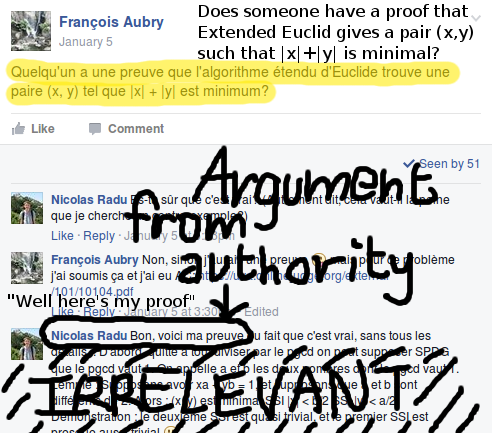
\includegraphics[width=.8\textwidth]{img/authority}
\end{center}
\end{frame}

\end{document}
